\section{Funciones de distancia con signo (FDS)}

\SectionPage

\subsection{Primitivas sobre \(\mathbb{R}^2\)}
\begin{frame}[fragile]{Primitivas sobre \(\mathbb{R}^2\)}
    
    Funciones de distancia con signo de \cite{2ddistinigo} y \cite{3ddistinigo},
    
    \begin{columns}[c, onlytextwidth]
        \column{1.5in}
            \begin{figure}[H]
              \centering
              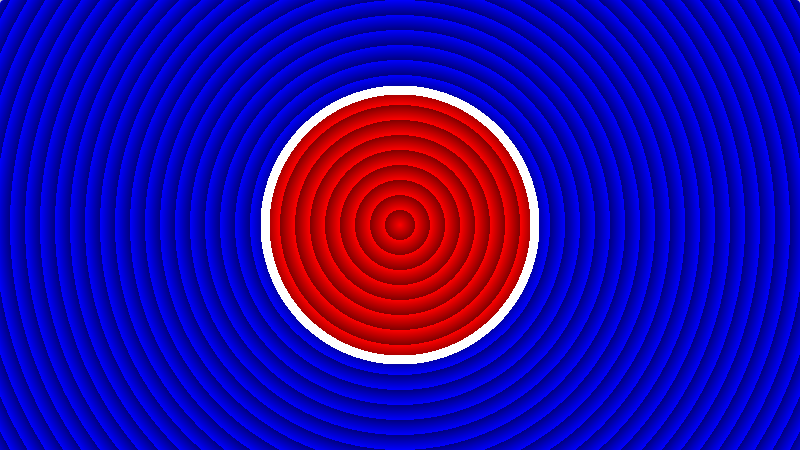
\includegraphics[width=1.0\textwidth]{imagenes/sdf/2d/sdf_circunsferencia.png}
            \end{figure}
        
        \column{\dimexpr\paperwidth-10pt}
        
            \begin{lstlisting}
    float SDFCircunsferencia(vec2 p, float r){
        return length(p) - r;
    }
            \end{lstlisting}
        
    \end{columns}
    
    \begin{columns}[c, onlytextwidth]
        \column{\dimexpr\paperwidth-140pt}
            \begin{lstlisting}
    float SDFRectangulo(vec2 p, vec2 s){
            vec2 a = abs(p) - s;
            float extr = length(max(a, 0.0));
            float intr = min(max(a.x, a.y), 0.0);
            return extr + intr;
    }
            \end{lstlisting}
    
        \column{1.5in}
            \begin{figure}[H]
              \centering
              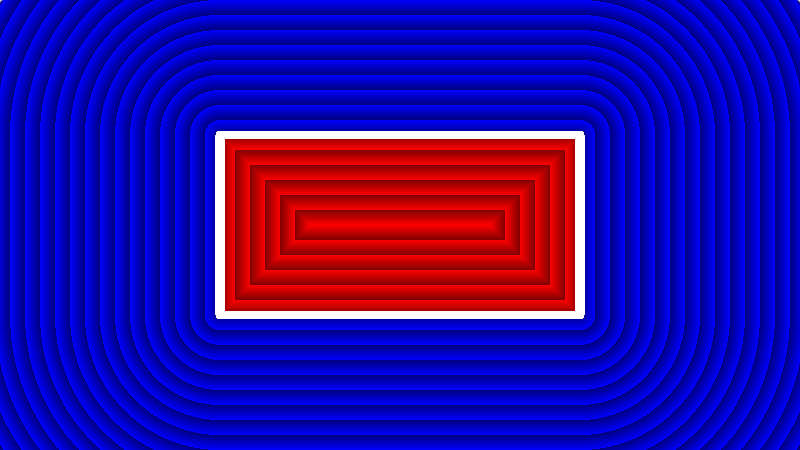
\includegraphics[width=1.0\textwidth]{imagenes/sdf/2d/sdf_rectangulo.png}
            \end{figure}
        
    \end{columns}
    
    \begin{columns}[c, onlytextwidth]
        \column{1.5in}
            \begin{figure}[H]
              \centering
              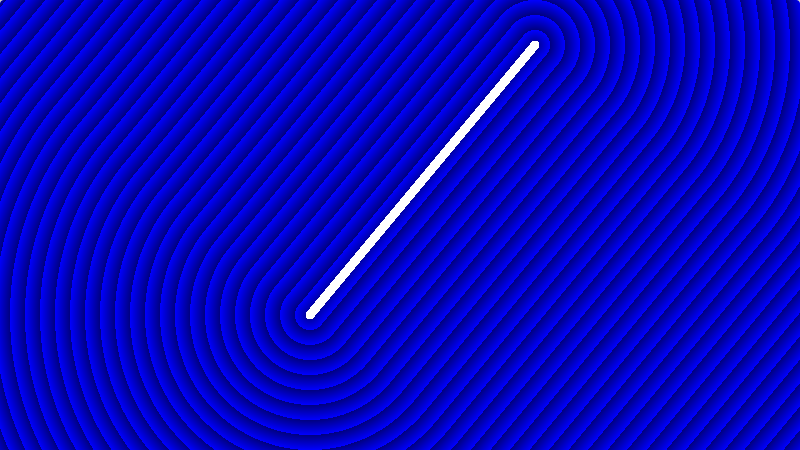
\includegraphics[width=1.0\textwidth]{imagenes/sdf/2d/sdf_segmento.png}
            \end{figure}
        
        \column{\dimexpr\paperwidth-10pt}
            \begin{lstlisting}
    vec2 proy01(in vec2 a, in vec2 b){
        return b * clamp(dot(b, a) / dot(b, b), 0., 1.);
    }
    float SDFSegmento(vec2 p, vec2 a, vec2 b){
        vec2 v = p - a;
        vec2 w = b - a;
        return length(v -  proy01(v, w));
    }
            \end{lstlisting}
        
    \end{columns}

\end{frame}

% PRIMITIVAS R2
\begin{frame}[fragile]{Operadores sobre \(\mathbb{R}^2\)}

    \begin{columns}[c, onlytextwidth]
        \column{1.5in}
            \begin{figure}[H]
              \centering
              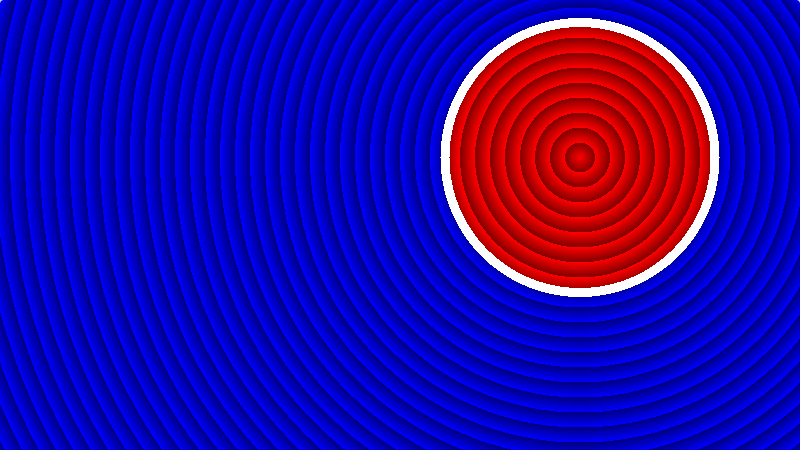
\includegraphics[width=1.0\textwidth]{imagenes/sdf/2d/sdf_traslacion.png}
            \end{figure}
        
        \column{\dimexpr\paperwidth-10pt}
        
            \begin{lstlisting}
                float escena_sdf(vec2 p){
                    vec2 pt = p - vec2(0.1, 0.2);
                    return SDFCircunsferencia(pt, 0.3);
                }
            \end{lstlisting}
        
    \end{columns}
    
    \begin{columns}[c, onlytextwidth]
        \column{\dimexpr\paperwidth-140pt}
            \begin{lstlisting}
    #define PI 3.1415
    mat2 rot(float a){
        return mat2(+cos(a), -sin(a), +sin(a), +cos(a));
    }
    float escena_sdf(vec2 p){
        vec2 pr = p * rot(45. * PI / 180.);
        return SDFRectangulo(pr, vec2(0.3));
    }
            \end{lstlisting}
    
        \column{1.5in}
            \begin{figure}[H]
              \centering
              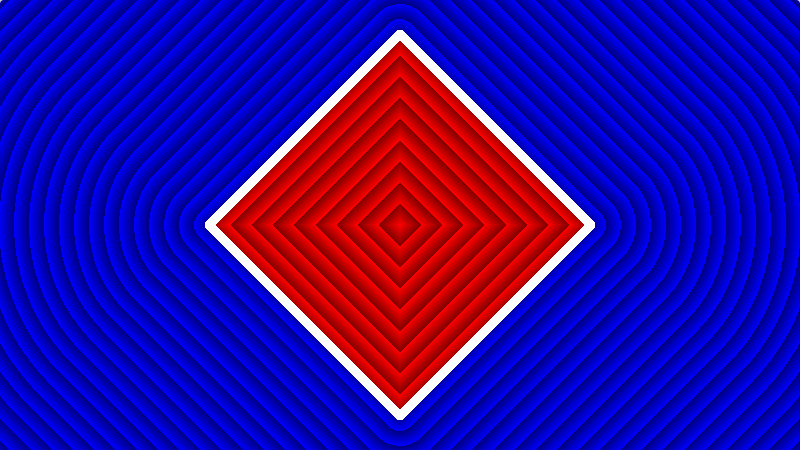
\includegraphics[width=1.0\textwidth]{imagenes/sdf/2d/sdf_rotacion.png}
            \end{figure}
        
    \end{columns}
    
    \begin{columns}[c, onlytextwidth]
        \column{1.5in}
            \begin{figure}[H]
              \centering
              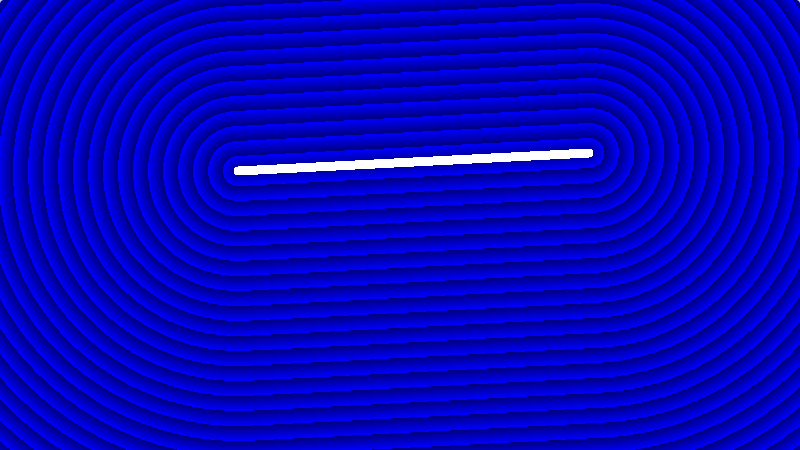
\includegraphics[width=1.0\textwidth]{imagenes/sdf/2d/sdf_simetria.png}
            \end{figure}
        
        \column{\dimexpr\paperwidth-10pt}
    \begin{lstlisting}
    vec2 simetria(vec2 p, vec2 a, vec2 b){
        return a + simetria(b - a, p - a);
    }
    float escena_sdf(vec2 p){
        vec2 a = vec2(0.2, 0.2), b = vec2(0.0, 0.1);
        vec2 ps = simetria(p, a, b);
        return SDFSegmento(ps, vec2(-0.2, -0.2), vec2(0.3, 0.4));
    }
            \end{lstlisting}
        
    \end{columns}

\end{frame}

% OPERADORES R2
\begin{frame}[fragile]{Operadores sobre \(\mathbb{R}^2\)}

    \begin{columns}[c, onlytextwidth]
        \column{1.5in}
            \begin{figure}[H]
              \centering
              
\includegraphics[width=1.0\textwidth]{imagenes/sdf/2d/sdf_add.png}
            \end{figure}
        
        \column{\dimexpr\paperwidth-10pt}
        
            \begin{lstlisting}
    float escena_sdf(vec2 p){
        vec2 pr = p * rot(PI / 180. * 45.0);
        vec2 pt = p - vec2(0.4, 0.15);
        return min(
            SDFRectangulo(pr, vec2(0.3)), // f
            SDFCircunsferencia(pt, 0.3)   // g
        );
    }
            \end{lstlisting}
        
    \end{columns}
    
    \begin{columns}[c, onlytextwidth]
        \column{\dimexpr\paperwidth-140pt}
            \begin{lstlisting}
    float escena_sdf(vec2 p){
        vec2 pr = p * rot(PI / 180. * 45.0);
        vec2 pt = p - vec2(0.4, 0.15);
        return max(
            SDFRectangulo(pr, vec2(0.3)),
            -SDFCircunsferencia(pt, 0.3)
        );
    }
            \end{lstlisting}
    
        \column{1.5in}
            \begin{figure}[H]
              \centering
              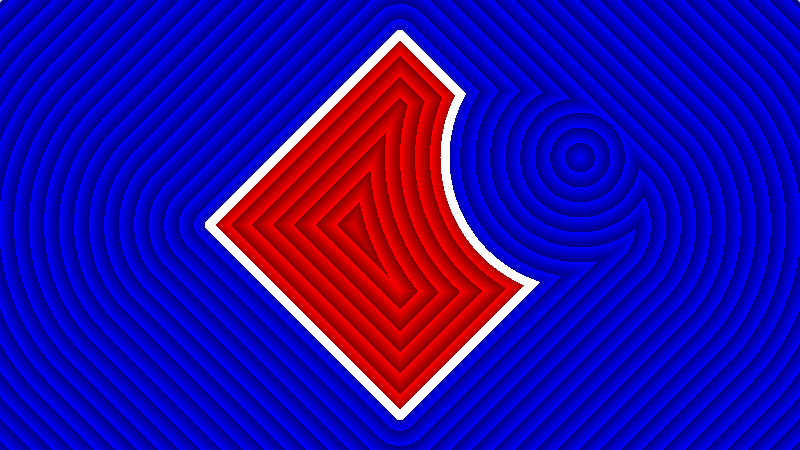
\includegraphics[width=1.0\textwidth]{imagenes/sdf/2d/sdf_subtract-3.png}
            \end{figure}
        
    \end{columns}
    
    \begin{columns}[c, onlytextwidth]
        \column{1.5in}
            \begin{figure}[H]
              \centering
              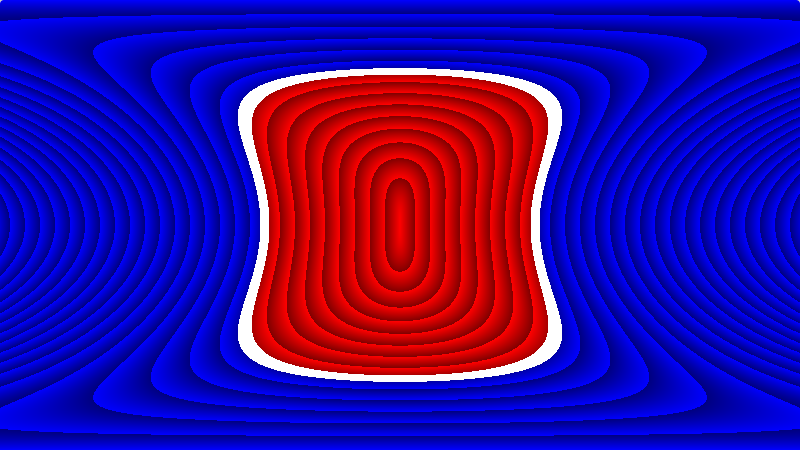
\includegraphics[width=1.0\textwidth]{imagenes/sdf/2d/sdf_deform.png}
            \end{figure}
        
        \column{\dimexpr\paperwidth-10pt}
            \begin{lstlisting}
    float sdf(vec2 p){
    	vec2 pn = vec2(
    	    p.x * cos(p.y * PI),
    	    p.y * sin(p.y * PI)
    	);
    	return SDFCircunferencia(pn, 0.1);
    }
            \end{lstlisting}
        
    \end{columns}

\end{frame}


\subsection{Primitivas sobre \(\mathbb{R}^3\)}
% OPERADORES R3
\begin{frame}[fragile]{Primitivas sobre \(\mathbb{R}^3\)}

    \begin{columns}[c, onlytextwidth]
        \column{1.5in}
            \begin{figure}[H]
              \centering
              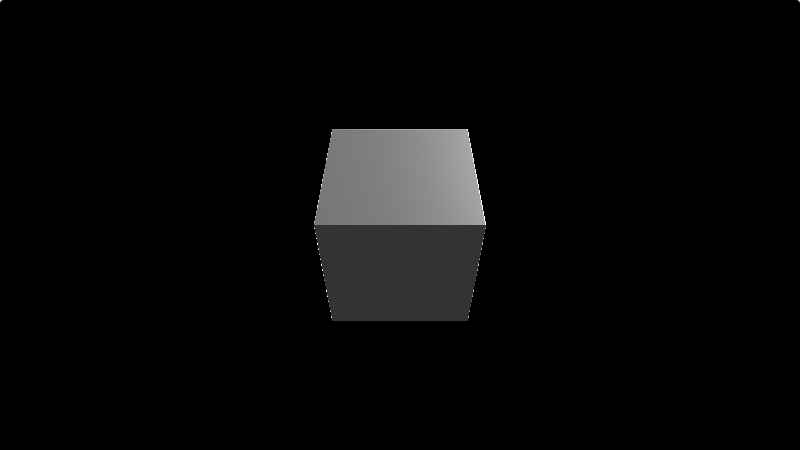
\includegraphics[width=1.0\textwidth]{imagenes/sdf/3d/sdf_prisma_rect.png}
            \end{figure}
        
        \column{\dimexpr\paperwidth-10pt}
        
            \begin{lstlisting}
    float SDFPrisma(vec3 p, vec3 s){
        vec3 pa = abs(p) - s;
        return length(max(pa, 0.)) +
        min(max(max(pa.x, pa.y), pa.z), 0.);
    }
            \end{lstlisting}
        
    \end{columns}
    
    \begin{columns}[c, onlytextwidth]
        \column{\dimexpr\paperwidth-140pt}
            \begin{lstlisting}
    float SDFPlano(vec3 p, vec3 n){
       return dot(p, n);
    }
            \end{lstlisting}
    
        \column{1.5in}
            \begin{figure}[H]
              \centering
              
\includegraphics[width=1.0\textwidth]{imagenes/sdf/3d/sdf_plano.png}
            \end{figure}
        
    \end{columns}
    
    \begin{columns}[c, onlytextwidth]
        \column{1.5in}
            \begin{figure}[H]
              \centering
              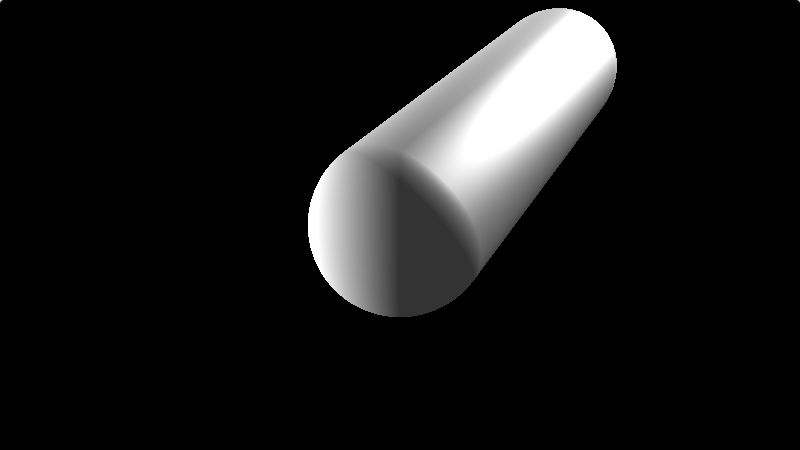
\includegraphics[width=1.0\textwidth]{imagenes/sdf/3d/sdf_capsula.png}
            \end{figure}
        
        \column{\dimexpr\paperwidth-10pt}
            \begin{lstlisting}
    float SDFSegmento(vec3 p, vec3 a, vec3 b){
        vec3 v = p - a;
        vec3 w = b - a;
        return length(v -  proy01(v, w));
    }
    float SDFCapsula(vec3 p, vec3 a, vec3 b, float k){
        return SDFSegmento(p, a, b) - k;
    }
            \end{lstlisting}
        
    \end{columns}

\end{frame}

\begin{frame}[fragile]{Operadores sobre \(\mathbb{R}^3\)}

    \begin{columns}[c, onlytextwidth]
        \column{1.5in}
            \begin{figure}[H]
              \centering
              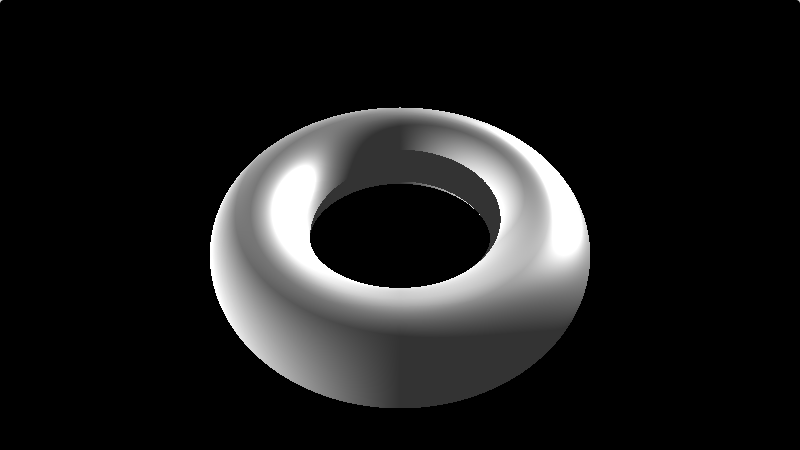
\includegraphics[width=1.0\textwidth]{imagenes/sdf/3d/sdf_toro.png}
            \end{figure}
        
        \column{\dimexpr\paperwidth-10pt}
        
            \begin{lstlisting}
    float SDFToro(vec3 p, float rx, float r){   
        vec2 rev = vec2(length(p.xz), p.y);
        vec2 pt = rev - vec2(rx, 0.);
        return SDFCircunferencia(pt, r);
    }
            \end{lstlisting}
        
    \end{columns}
    
    \begin{columns}[c, onlytextwidth]
        \column{\dimexpr\paperwidth-140pt}
            \begin{lstlisting}
    float SDFCilindro(vec3 p, float r){
        vec3 n = normalize(vec3(1, 0, 0));
        vec2 proy = proyPlano(p, n).yz;
        return SDFCircunferencia(proy, r);
    }
            \end{lstlisting}
    
        \column{1.5in}
            \begin{figure}[H]
              \centering
              
\includegraphics[width=1.0\textwidth]{imagenes/sdf/3d/sdf_cilindro_infinito.png}
            \end{figure}
        
    \end{columns}
    
    \begin{columns}[c, onlytextwidth]
        \column{1.5in}
            \begin{figure}[H]
              \centering
              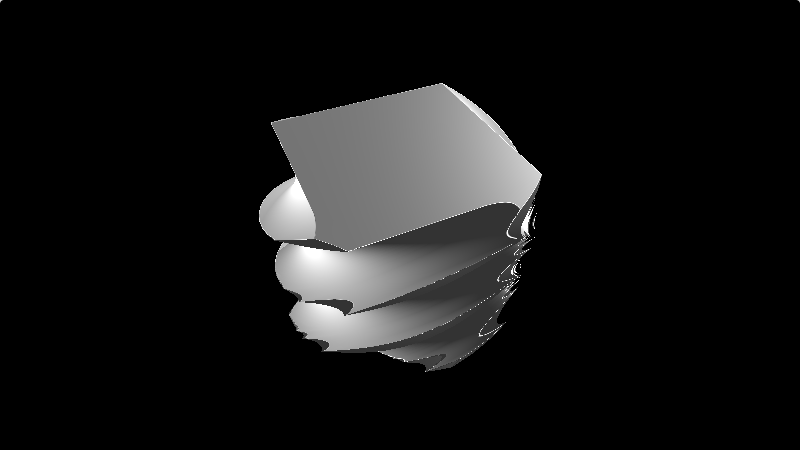
\includegraphics[width=1.0\textwidth]{imagenes/sdf/3d/sdf_twist.png}
            \end{figure}
        
        \column{\dimexpr\paperwidth-10pt}
            \begin{lstlisting}
    float escena_sdf(vec3 p){
        vec2 ry = p.yz * rot(PI / 4.0);
        p = vec3(p.x, ry.x, ry.y);
        float a = p.y * 10.0;
        p = vec3(
            +p.x * cos(a) + p.z * sin(a),
            +p.y,
            -p.x * sin(a) + p.z * cos(a)
        );
        p.xz * rot(a)
        return SDFPrisma(p, vec3(0.2));
    }
            \end{lstlisting}
        
    \end{columns}

\end{frame}